
\begin{frame}
  \frametitle<1>{FeS$_2$: Single scattering paths in a crystal}
  \frametitle<2>{FeS$_2$: Multiple scattering paths in a crystal}
  \begin{columns}[T]
    \begin{column}{0.6\linewidth}
      \begin{center}
        \includegraphics<1>[width=0.6\linewidth]{images/FeS2/fes2}
        \includegraphics<2>[width=0.9\linewidth]{images/FeS2/intrp}
      \end{center}

      \begin{onlyenv}<1>
        \small
        {\color{Chocolate3}$\bullet$} = Fe \quad%
        {\color{Gold2}$\bullet$} = S

        The first sulfur SS path is from the octahedron surrounding
        the Fe atom.  It provides most of the spectral weight under
        the first peak.

        The next two S and one Fe SS paths overlap between 2.5 and
        3.5\,\AA.
      \end{onlyenv}
      \begin{onlyenv}<2>
        \small
        The relationship between the EXAFS spectrum and atomic
        structure can be quite complicated due to multiple
        scattering.

        S--S and S--Fe triangles contribute
        significantly between 2.5 and 3.5\,\AA.
      \end{onlyenv}
    \end{column}
    %%
    \begin{column}{0.4\linewidth}
      \includegraphics<1>[width=\linewidth]{images/FeS2/fourss}
      \includegraphics<2>[width=\linewidth]{images/FeS2/fourms}

      \bigskip

      \includegraphics<1>[width=\linewidth]{images/FeS2/fourss_re}
      \includegraphics<2>[width=\linewidth]{images/FeS2/fourms_re}

      \bigskip

      ~

      \bigskip
    \end{column}
  \end{columns}
  \begin{textblock*}{0.5\linewidth}(0pt,20\TPVertModule) 
    \tiny
    Data from
    \href{http://cars9.uchicago.edu/~newville/ModelLib}
    {\color{Purple4}\texttt{http://cars9.uchicago.edu/~newville/ModelLib}}
  \end{textblock*}
\end{frame}

\begin{frame}
  \frametitle{[Ni(CN)$_4$]$^{2-}$: Paths in a molecule}
  \begin{columns}
    \begin{column}{6cm}
      \begin{center}
        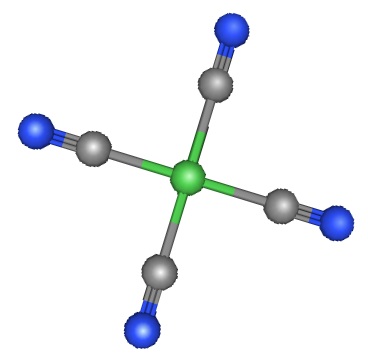
\includegraphics[width=3cm]{images/NiCN/nicn}

        {\color{Green4}$\bullet$} = Ni\quad
        {\color{Gray0}$\bullet$} = C\quad
        {\color{Blue2}$\bullet$} = N
      \end{center}
      Multiple scattering is \textbf{not} just for the materials
      scientists.  [Ni(CN)$_4$]$^{2-}$ in solution is \textbf{not} a
      crystal.

      Without consideration of the MS paths, the huge second peak in
      these data cannot be fit.
    \end{column}
    %%
    \begin{column}{4cm}
      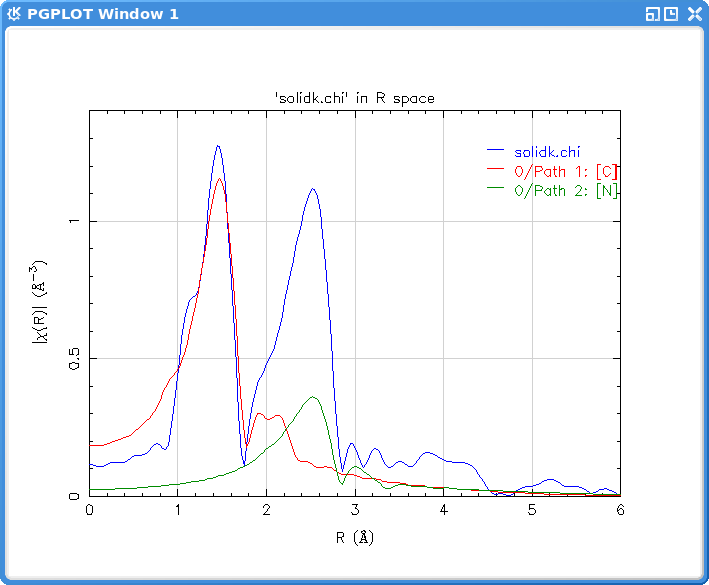
\includegraphics[width=\linewidth]{images/NiCN/ss}

      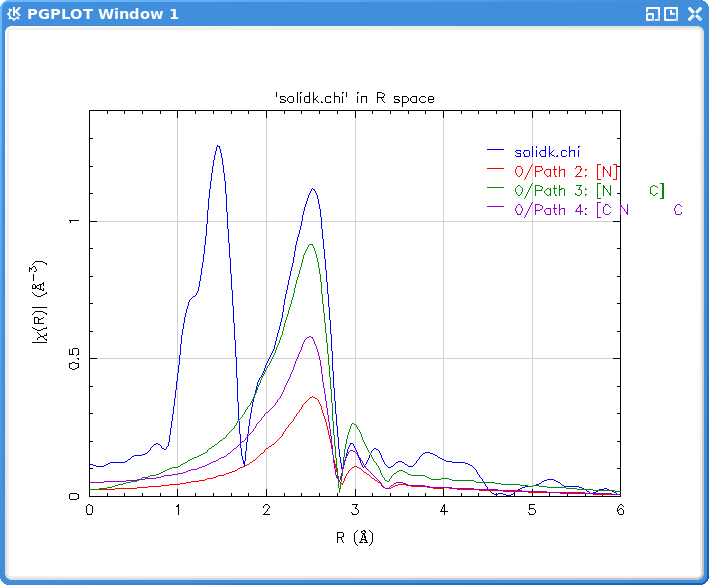
\includegraphics[width=\linewidth]{images/NiCN/ms}
    \end{column}
  \end{columns}
  \begin{textblock*}{0.5\linewidth}(0pt,20\TPVertModule) 
    \tiny
    A.\ Mu\~noz-P\'aez et al. Inorg.\ Chem. \textbf{39} (2000) pp.\ 3784--3790
  \end{textblock*}
\end{frame}

%%% Local Variables:
%%% mode: latex
%%% TeX-master: "pimst2"
%%% End:
